%=======================02-713 LaTeX template, following the 15-210 template==================
%
% You don't need to this template
%
\documentclass[11pt]{article}
\usepackage{amsmath,amssymb,amsthm}
\usepackage{graphicx}
\usepackage{wrapfig}
\usepackage[margin=1in]{geometry}
\usepackage{fancyhdr}
\setlength{\parindent}{0pt}
\setlength{\parskip}{5pt plus 1pt}
\setlength{\headheight}{13.6pt}
\newcommand\question[2]{\vspace{.25in}\hrule\textbf{#1: #2}\vspace{.5em}\hrule\vspace{.10in}}
\renewcommand\part[1]{\vspace{.10in}\textbf{(#1)}}
\newcommand\algorithm{\vspace{.10in}\textbf{Algorithm: }}
\newcommand\correctness{\vspace{.10in}\textbf{Correctness: }}
\newcommand\runtime{\vspace{.10in}\textbf{Running time: }}
\newcommand\tab[1][1cm]{\hspace*{#1}}
\pagestyle{fancyplain}
\lhead{\textbf{\NAME\ (\ANDREWID)}}
\chead{\textbf{HW\HWNUM}}
\rhead{02-713, \today}
\begin{document}\raggedright
%Section A==============Change the values below to match your information==================
\newcommand\NAME{Kadir Emre Otod}  % your name
\newcommand\ANDREWID{150140032}     % your andrew id
\newcommand\HWNUM{4}              % the homework number
%Section B==============Put your answers to the questions below here=======================

% no need to restate the problem --- the graders know which problem is which,
% but replacing "The First Problem" with a short phrase will help you remember
% which problem this is when you read over your homeworks to study.

\question{1}{Single Channel AM Communication System} 

\begin{figure}[h]
	\centering
	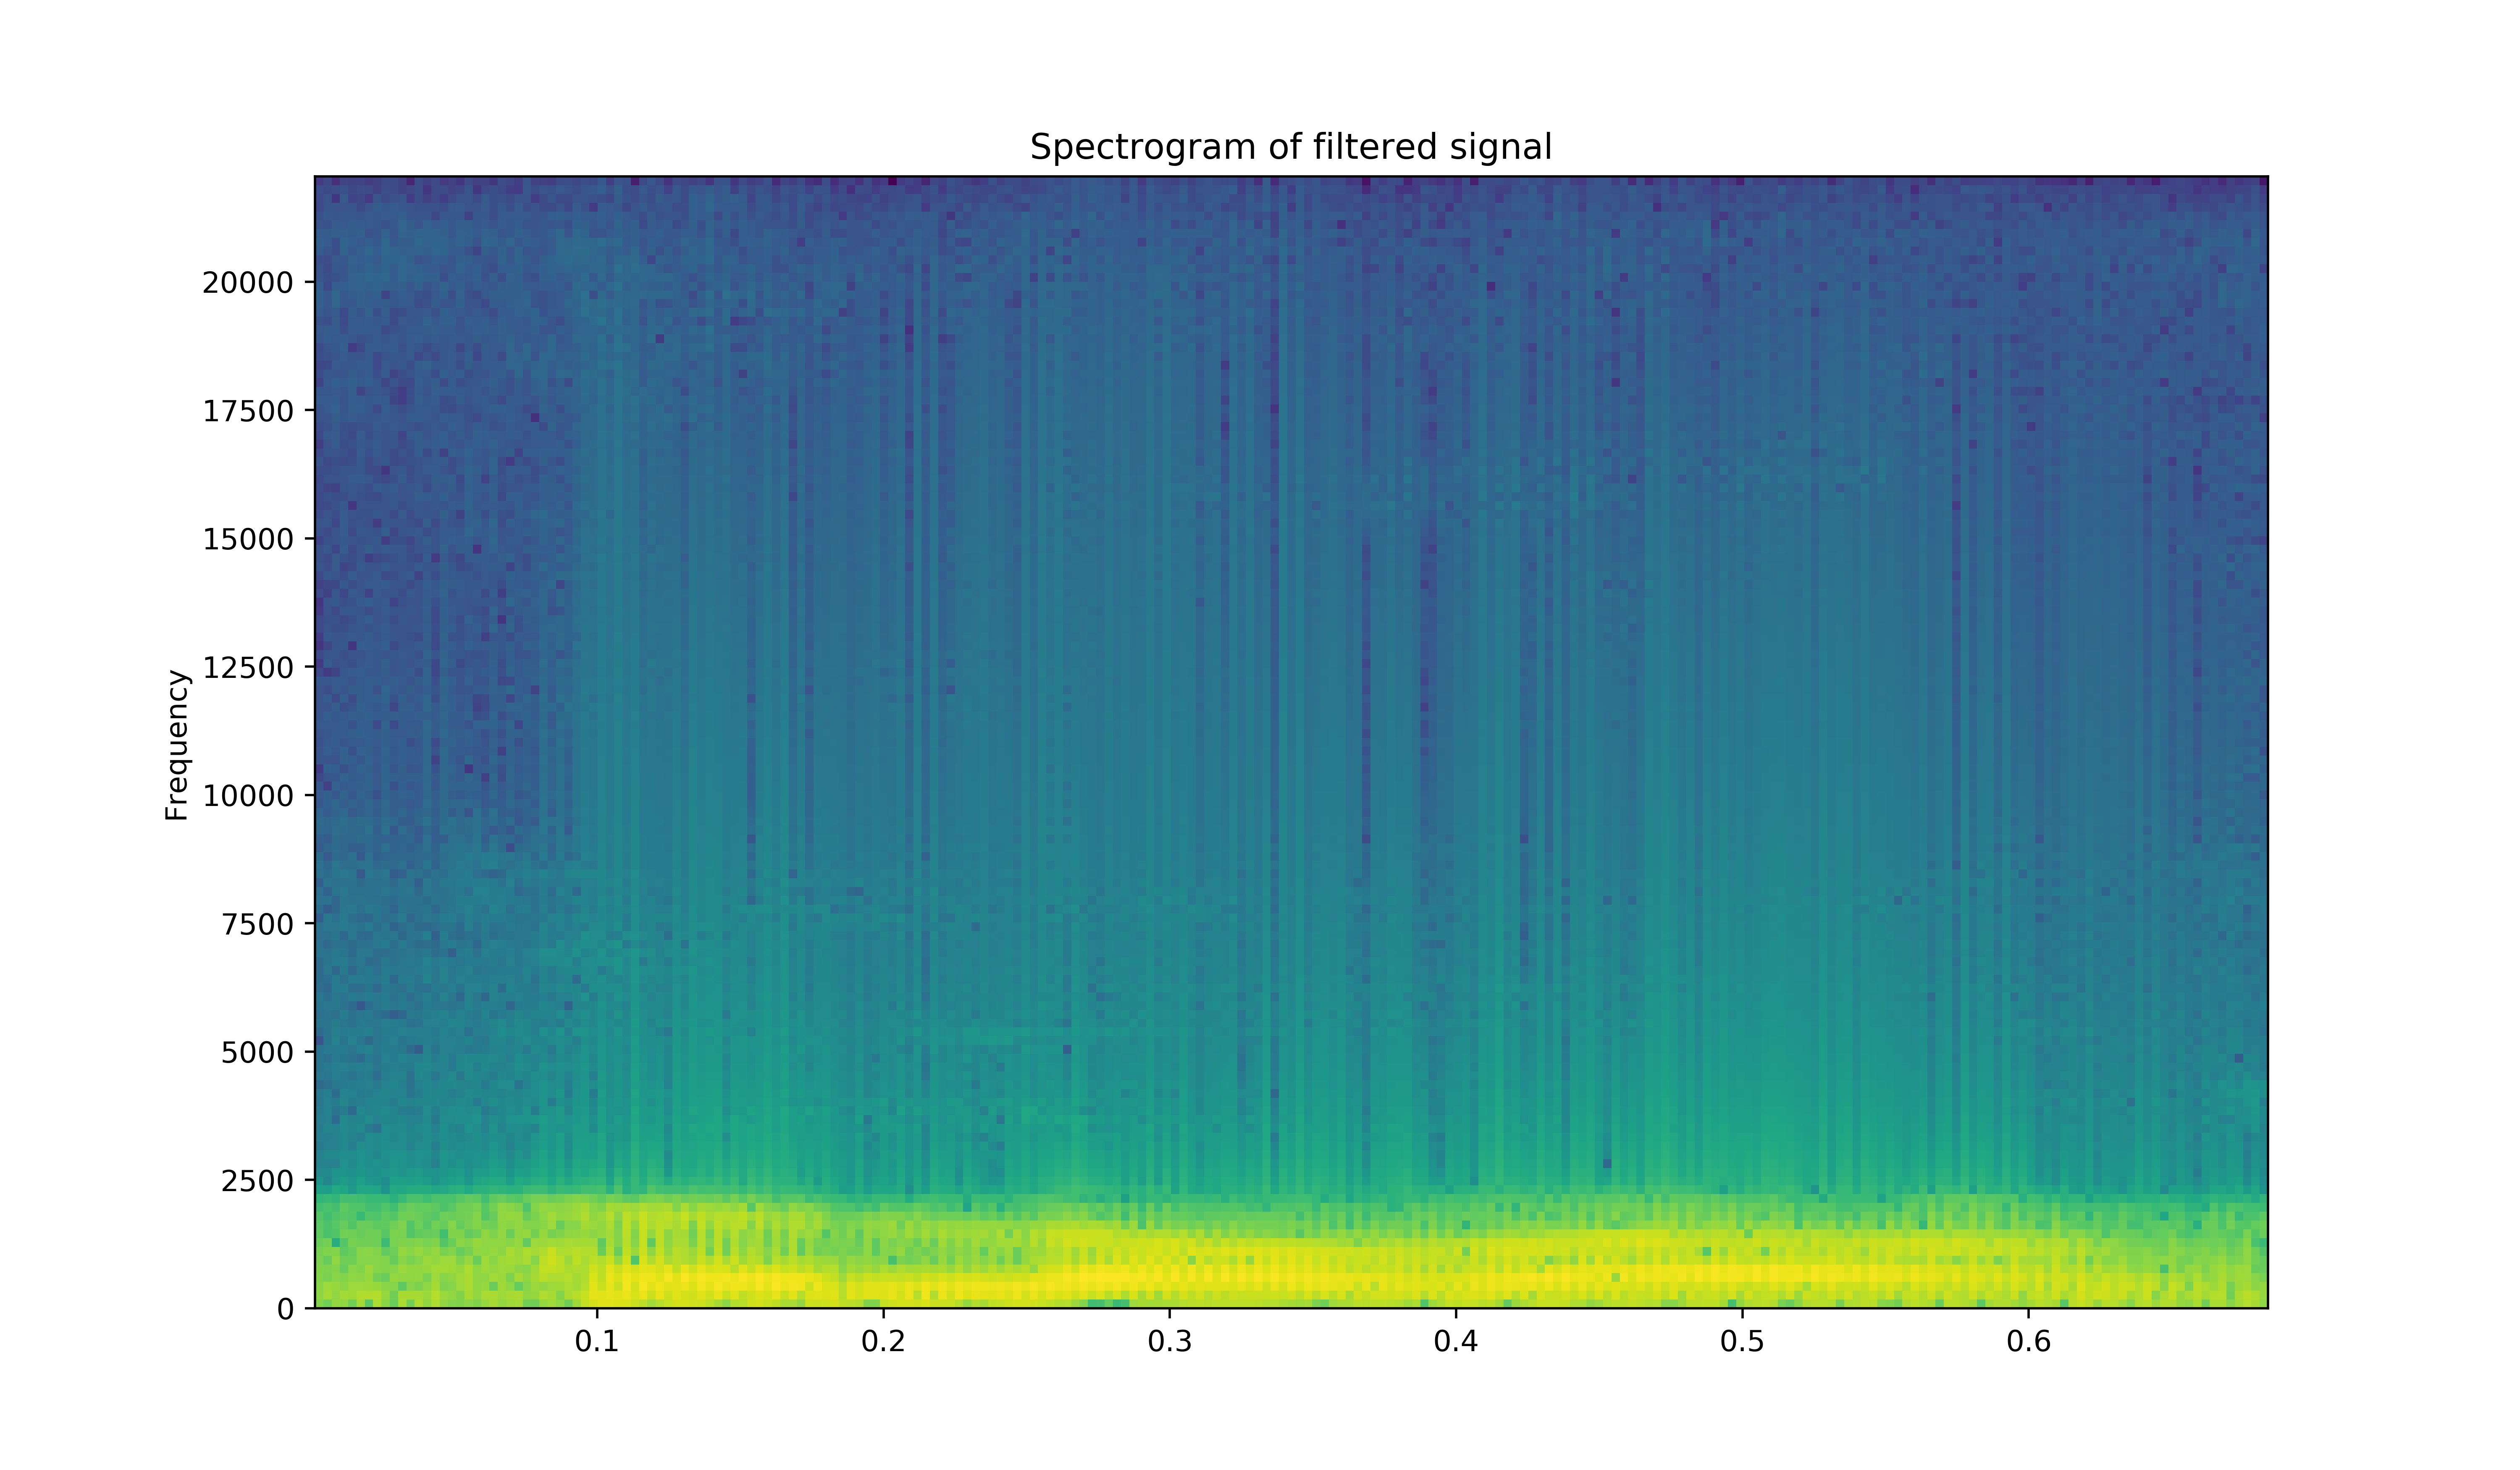
\includegraphics[width=0.8\linewidth]{figure-3}
	\caption{Spectrogram of filtered signal}
\end{figure}

The display of the spectrogram is given at Figure 1. I can estimate the bandwidth of the speech signal $\left[0, 2500Hz\right]$

\begin{figure}[h]
	\centering
	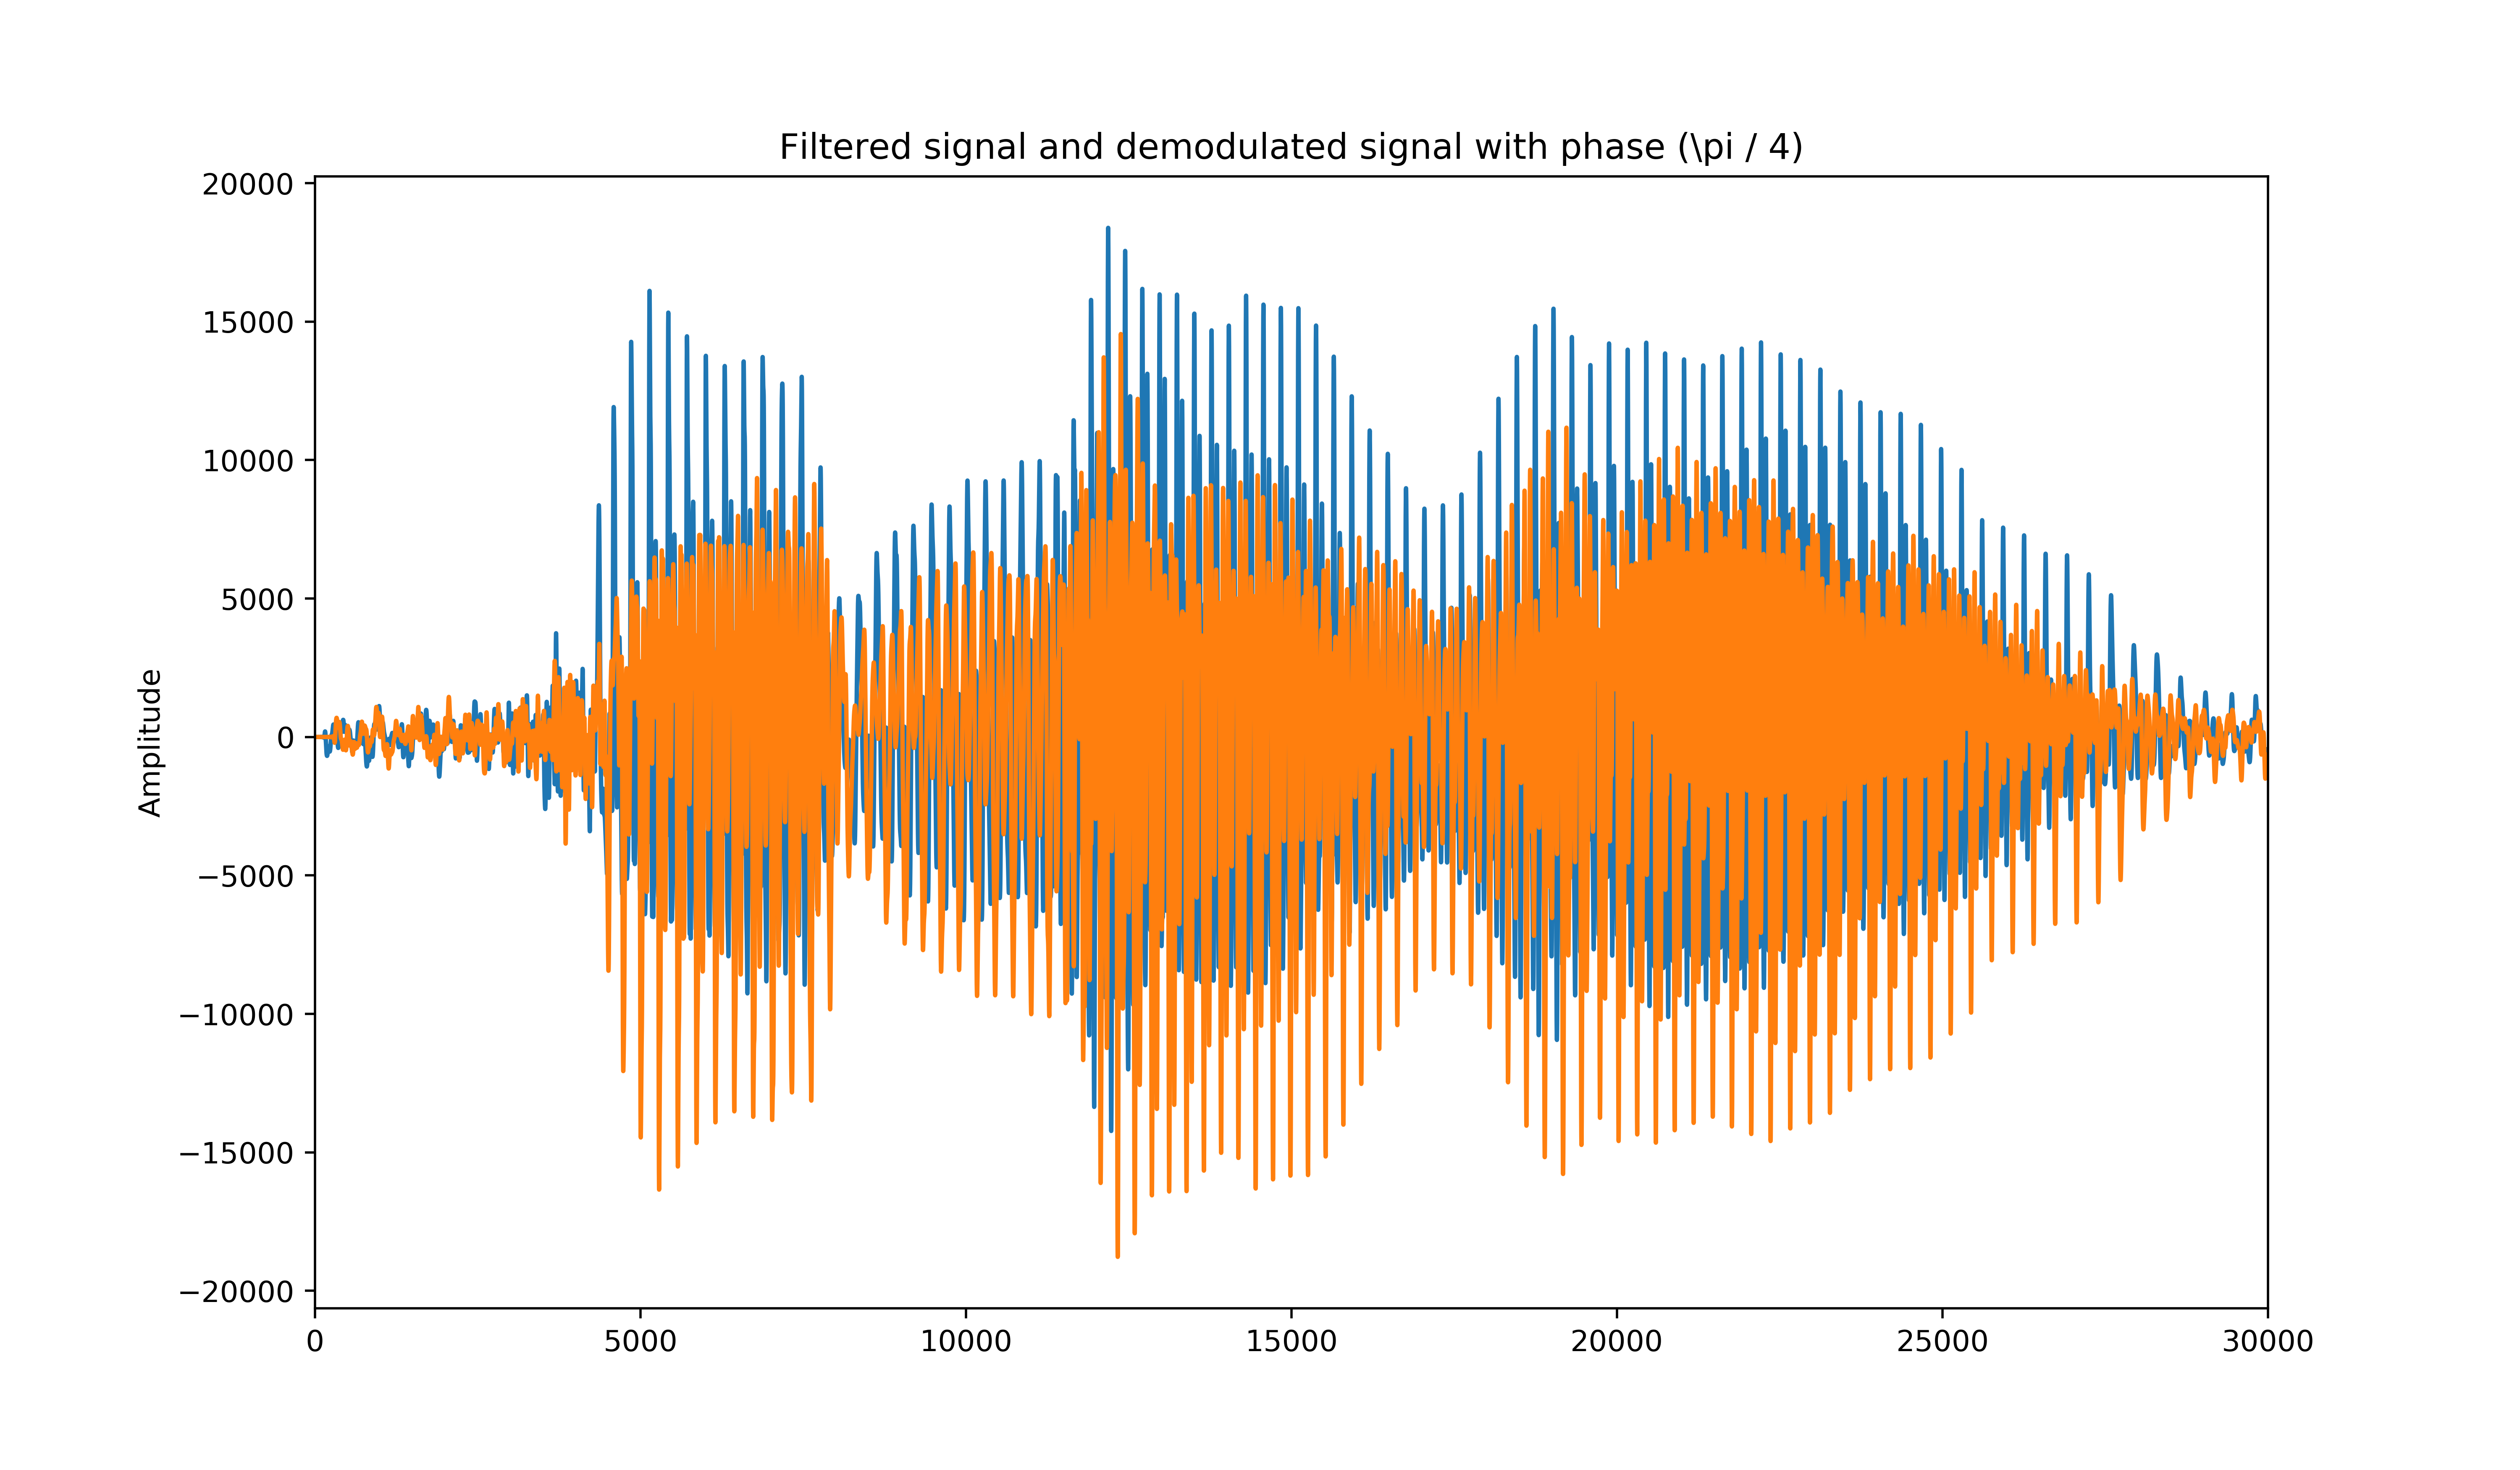
\includegraphics[width=0.8\linewidth]{figure-1}
	\caption{Filtered signal and demodulated signal with phase, $\pi / 2$}
\end{figure}


\begin{figure}[h]
	\centering
	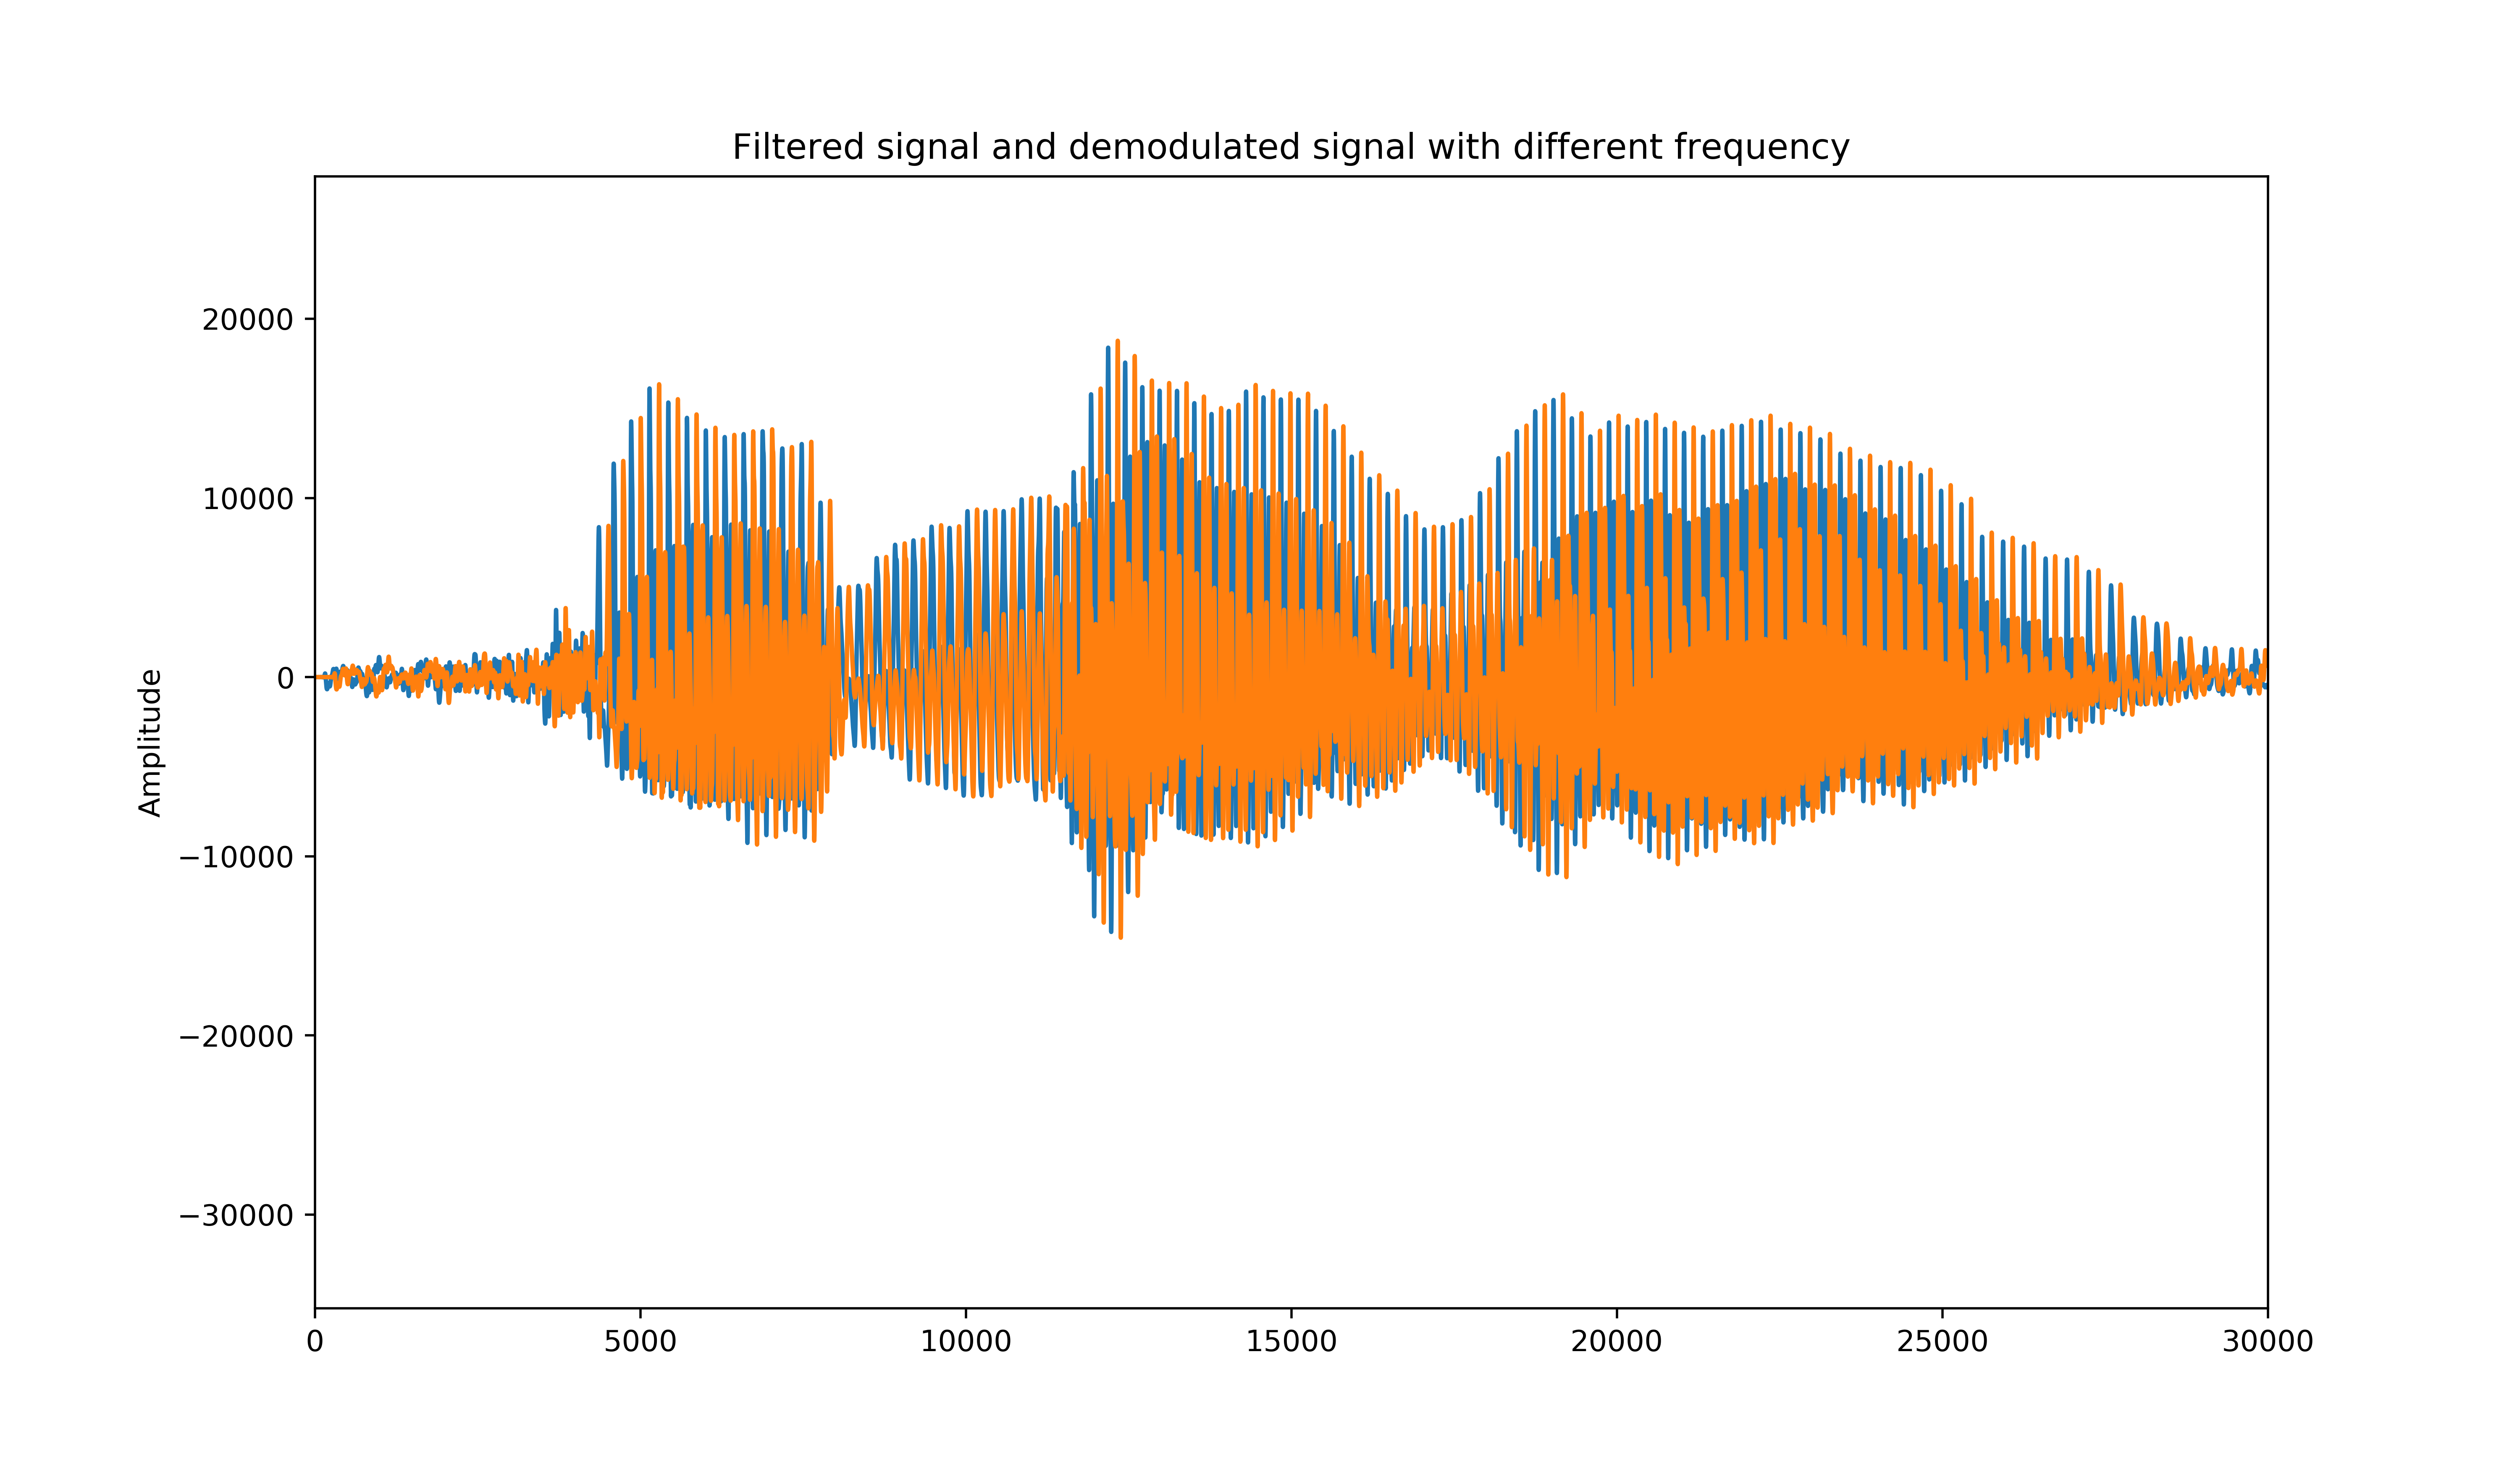
\includegraphics[width=0.8\linewidth]{figure-2}
	\caption{Filtered signal and demodulated signal with different frequency, +10 Hz}
\end{figure}

It is possible to say, if we add a phase ($\pi / 2$) to demodulator without changing carrier frequency, the applitude of demodulated signal reduces. (check figure 2)

If we add 10 Hz to the carrier frequency with zero phase, the amplitude does not change at all. (check figure 3)

\end{document}
